% Flywheel diagram – PPT colour scheme
% Compile with: xelatex flywheel_ppt_colors.tex
% Convert with: dvisvgm --pdf flywheel_ppt_colors.pdf -o flywheel_ppt_colors_tikz.svg
\documentclass[border=10pt]{standalone}
\usepackage{fontspec}
\setmainfont{Aptos}[
  Path = /Applications/Microsoft Word.app/Contents/Resources/DFonts/,
  Extension = .ttf,
  UprightFont = Aptos,
  BoldFont = Aptos-Bold,
  ItalicFont = Aptos-Italic,
  BoldItalicFont = Aptos-Bold-Italic,
]
\usepackage{tikz}
\usetikzlibrary{arrows.meta, positioning, decorations.markings, calc}

% Colours from the PPT SVG
\definecolor{boxfill}{HTML}{0D0D0D}      % rgba(255,255,255,0.05) on dark bg
\definecolor{boxstroke}{HTML}{2A2A2A}     % rgba(255,255,255,0.1)
\definecolor{accent}{HTML}{CB8044}        % arrows and markers
\definecolor{heading}{HTML}{E8E8E8}       % box headings
\definecolor{subtext}{HTML}{AAAAAA}       % descriptions and labels
\definecolor{bg}{HTML}{1A1A1A}           % dark background

\begin{document}
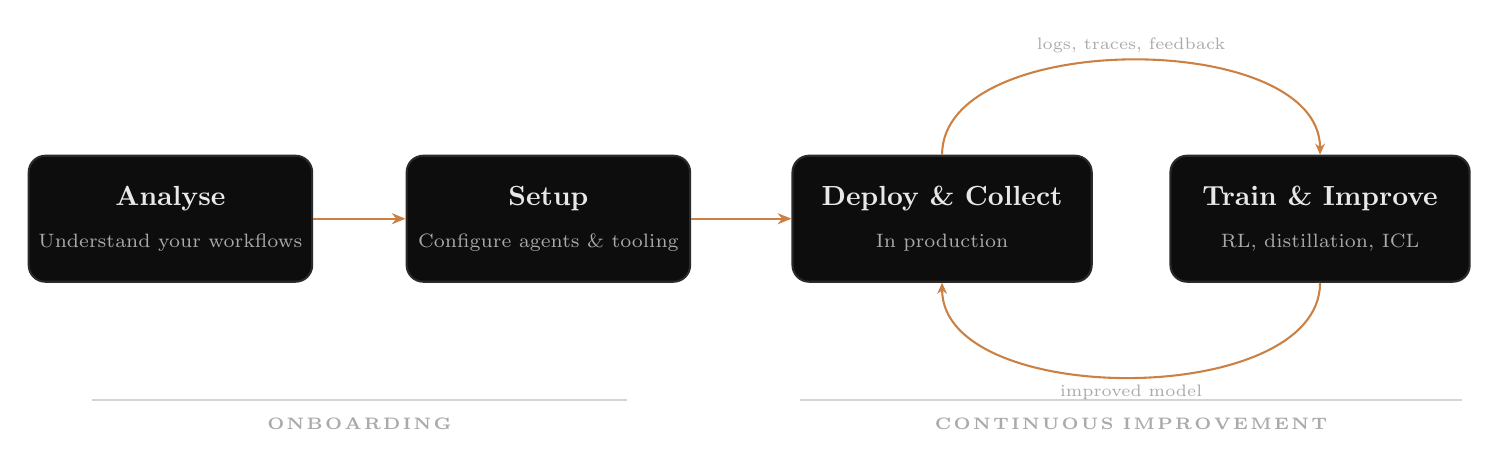
\begin{tikzpicture}[
    >=Stealth,
    box/.style={
        rectangle,
        rounded corners=6pt,
        minimum width=3.6cm,
        minimum height=1.6cm,
        draw=boxstroke,
        line width=0.75pt,
        fill=boxfill,
        align=center,
    },
    arrowline/.style={
        accent,
        line width=0.75pt,
        -{Stealth[length=5pt, width=4pt]},
    },
    curvedarrow/.style={
        accent,
        line width=0.75pt,
        -{Stealth[length=4pt, width=3.5pt]},
    },
]

% No background fill – transparent

% Boxes
\node[box] (analyse) at (0,0) {
    \textcolor{heading}{\fontsize{10}{12}\selectfont\bfseries Analyse}\\[3pt]
    \textcolor{subtext}{\fontsize{7}{9}\selectfont Understand your workflows}
};

\node[box] (setup) at (4.8,0) {
    \textcolor{heading}{\fontsize{10}{12}\selectfont\bfseries Setup}\\[3pt]
    \textcolor{subtext}{\fontsize{7}{9}\selectfont Configure agents \& tooling}
};

\node[box, minimum width=3.8cm] (deploy) at (9.8,0) {
    \textcolor{heading}{\fontsize{10}{12}\selectfont\bfseries Deploy \& Collect}\\[3pt]
    \textcolor{subtext}{\fontsize{7}{9}\selectfont In production}
};

\node[box, minimum width=3.8cm] (train) at (14.6,0) {
    \textcolor{heading}{\fontsize{10}{12}\selectfont\bfseries Train \& Improve}\\[3pt]
    \textcolor{subtext}{\fontsize{7}{9}\selectfont RL, distillation, ICL}
};

% Straight arrows between boxes
\draw[arrowline] (analyse.east) -- (setup.west);
\draw[arrowline] (setup.east) -- (deploy.west);

% Top curved arrow: Deploy -> Train
\draw[curvedarrow]
    (deploy.north) .. controls ++(0,1.6) and ++(0,1.6) .. (train.north);
\node[subtext, font=\fontsize{6.5}{8}\selectfont] at (12.2,2.2) {logs, traces, feedback};

% Bottom curved arrow: Train -> Deploy
\draw[curvedarrow]
    (train.south) .. controls ++(0,-1.6) and ++(0,-1.6) .. (deploy.south);
\node[subtext, font=\fontsize{6.5}{8}\selectfont] at (12.2,-2.2) {improved model};

% Bottom labels
\node[subtext, font=\fontsize{6}{8}\selectfont\bfseries] at (2.4,-2.6) {O\kern0.1em N\kern0.1em B\kern0.1em O\kern0.1em A\kern0.1em R\kern0.1em D\kern0.1em I\kern0.1em N\kern0.1em G};
\node[subtext, font=\fontsize{6}{8}\selectfont\bfseries] at (12.2,-2.6) {C\kern0.1em O\kern0.1em N\kern0.1em T\kern0.1em I\kern0.1em N\kern0.1em U\kern0.1em O\kern0.1em U\kern0.1em S\kern0.3em \kern0.1em I\kern0.1em M\kern0.1em P\kern0.1em R\kern0.1em O\kern0.1em V\kern0.1em E\kern0.1em M\kern0.1em E\kern0.1em N\kern0.1em T};

% Bracket lines for labels
\draw[subtext, line width=0.5pt, opacity=0.5] (-1.0,-2.3) -- (5.8,-2.3);
\draw[subtext, line width=0.5pt, opacity=0.5] (8.0,-2.3) -- (16.4,-2.3);

\end{tikzpicture}
\end{document}
